\chapter{La diffraction}
\begin{wrapfigure}[8]{r}{2cm}
\vspace{-6mm}
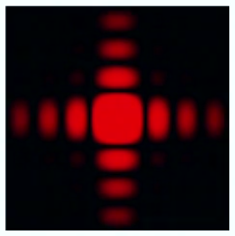
\includegraphics[scale=0.30]{ch2/image4.png}
\captionof{figure}{ }
\end{wrapfigure}
Un faisceau laser se propageant à tendance à s'élargir et se déformer : il s'agit du 
phénomène de diffraction. Ce phénomène est bien précis et peut être décrit mathématiquement. 
Il dépend notamment de la forme du laser. En faisant passer un laser par une section carrée, 
on sera amener à observer des distributions d'intensités particulières.

\section{Équations de Maxwell et transformée de Fourier}
La linéarité des équations de Maxwell permet un traitement efficace par les transformées 
de Fourier. Voici les fameuses équations dans le vide
\begin{equation}
\left\{\begin{array}{llll}
\rot \vec{E} &= -\dfrac{\partial \vec{B}}{\partial t},\qquad &\div \vec{E} &= 0\\
\rot \vec{B} &= \epsilon_0\mu_0\dfrac{\partial \vec{E}}{\partial t},\qquad &\div \vec{B} &= 0
\end{array}\right.
\end{equation}
Sachant que $\rot [\rot \vec{E}] = \grad[\div \vec{E}] - \Delta\vec{E}$ où $\div \vec{E}=0$ dans 
le vide on retrouve l'équation d'onde électromagnétique
\begin{equation}
\Delta \vec{E} = \mu_0\epsilon_0\dfrac{\partial^2\vec{E}}{\partial t^2}\quad \text{où } \Delta 
\vec{E} = \Delta E_x\vec{1_x}+\Delta E_y\vec{1_y}+\Delta E_z\vec{1_z}
\end{equation}
On ne considérera ici que la composante en $x$ du champ
\begin{equation}
\Delta E_x = \mu_0\epsilon_0\dfrac{\partial^2E_x}{\partial t^2}
\end{equation}
On remplacera souvent $E_x,E_y$ ou $E_z$ par $E$ mais il faut garder à l'idée qu'il ne s'agit 
qu'une seule des composantes du champ. L'équation d'onde scalaire s'écrit
\begin{equation}
\dfrac{\partial E}{\partial x^2}+\dfrac{\partial E}{\partial y^2}+\dfrac{\partial E}{\partial z^2} 
= \mu_0\epsilon_0\dfrac{\partial^2E}{\partial t^2}
\end{equation}
Cette équation est \textit{linéaire}, $E$ n'apparaissant qu'à la première puissance. Si $E_1$ et 
$E_2$ sont solution, une combili de ces deux solutions est également solution. On va profiter 
de cette linéarité pour exprimer la solution de cette équation comme une somme d'onde harmonique, 
d'où l'utilité des transformée de Fourier. Le champ électrique se verra décomposé en une somme 
de \textit{fonctions harmonique}\footnote{Écrit ci-dessous dans le domaine des phaseurs.} :
\begin{equation}
E(x,y,z,t) = \iiiint_{-\infty}^\infty \tilde{E}(k_x,k_y,k_z,\omega)e^{ik_xx}e^{ik_yy}e^{ik_zz}
e^{-i\omega t}\ dk_xdk_ydk_zd\omega
\end{equation}
Si le facteur harmonique $e^{ik_xx}e^{ik_yy}e^{ik_zz}e^{-i\omega t}$  est solution des équations 
de Maxwell $\forall k_i,\omega$, alors $E$ sera solution. La résolution de ces équations ne sont 
pas aisées. Pour le faire de façon analytique, on travaillera avec la décomposition. Vérifions 
que ces fonctions harmoniques sont bien solution
\begin{equation}
\dfrac{\partial^2 e^{ik_xx}e^{ik_yy}e^{ik_zz}e^{-i\omega t}}{\partial x^2} = -k_x^2 e^{ik_xx}e^{ik_yy}
e^{ik_zz}e^{-i\omega t}
\end{equation}
En faisant de même pour les deux autres dérivées partielles pour obtenir
\begin{equation}
(-k_x^2-k_y^2-k_z^2)e^{ik_xx}e^{ik_yy}e^{ik_zz}e^{-i\omega t} = -\mu_0\epsilon_0\omega^2 
e^{ik_xx}e^{ik_yy}e^{ik_zz}e^{-i\omega t}
\end{equation}
C'est-à-dire
\begin{equation}
k_x^2+k_y^2+k_z^2 = \mu_0\epsilon_0\omega^2
\end{equation}
Il s'agit d'une \textbf{contrainte} sur les modes de Fourier. On peut voir l'expression de $E$ 
comme une transformée de Fourier où $\tilde{E}$ est le spectre de Fourier généralisé à 4 
dimensions. En terme de transformée de Fourier, on peut dire qu'il s'agit d'une contrainte 
sur les \textit{modes de Fourier} (les quatre facteurs exponentiels), soit une \textbf{relation 
de dispersion généralisée}. Si les modes satisfont cette contrainte, $E$ sera solution.\\

\begin{wrapfigure}[9]{r}{3cm}
%\vspace{-6mm}
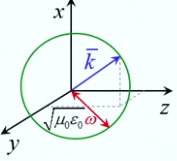
\includegraphics[scale=0.45]{ch2/image5.png}
\captionof{figure}{ }
\end{wrapfigure}
Intéressons-nous aux aspects physiques sous-jacent à cette décomposition de Fourier du champ 
électrique. Commençons par la ré-écriture suivante en supposant que les $k_i$ sont les 
composantes d'un vecteur
\begin{equation}
\tilde{E}(k_x,k_y,k_z,\omega)e^{ik_xx}e^{ik_yy}e^{ik_zz}e^{-i\omega t} = \tilde{E}(\vec{k},
\omega)e^{i\vec{k}.\vec{r}}e^{-i\omega t}
\end{equation}
\danger $\vec{r}$ est le vecteur position, il désigne le point de l'espace considéré. On peut 
ainsi exprimer la condition pour laquelle le mode de Fourier satisfait les équations de Maxwell  :
\begin{equation}
|k|^2 = k^2 = \mu_0\epsilon_0\omega^2
\end{equation}

\begin{wrapfigure}[9]{l}{3cm}
\vspace{-6mm}
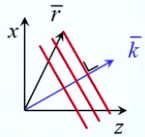
\includegraphics[scale=0.45]{ch2/image6.png}
\captionof{figure}{ }
\end{wrapfigure}
Cela signifie que le vecteur d'onde est tendu d'être sur une sphère de rayon $k=
\sqrt{\mu_0\epsilon_0}\omega$. Figeons le temps et cherchons le lieux des points de phase 
constante. Pour avoir une phase constante, $\vec{k}.\vec{r}$ doit être constant : tous les 
points qui ont la même projection auront la même phase, il s'agit d'une \textit{onde plane}.
Ci-contre, la représentation des fronts d'ondes. Analysons cela de façon analytique
\begin{equation}
\varphi = \vec{k}.\vec{r} = \text{cste}\quad \Rightarrow k_xx+k_yy+k_zz = \text{ cste}
\end{equation}
Il s'agit de l’équation d'un plan perpendiculaire au vecteur d'onde. Les modes de Fourier 
réprésentent bien une onde plane dont la direction $\vec{k}/k$. On peut toujours considérer 
$\vec{k}/k = \vec{1_z} \rightarrow \vec{k}= k\vec{1_z}$ de sorte à écrire
\begin{equation}
E = \tilde{E}e^{ikz}e^{-i\omega t}
\end{equation}
Ceci montre que lorsque $z$ est fixé, le champ ne varie pas en $x$. Si l'on considère la 
partie réelle de ceci, on retrouve $\tilde{E}\cos(kz-\omega t)$ ce qui est bien l'équation 
d'une onde plane.\\

Que se passe-t-il si on libère le temps? Intéressons-nous d'abord à la périodicité en 
$z : \lambda = 2\pi/k$ ce qui correspond à l'espacement des fronts d'ondes. Considérons 
une phase constante
\begin{equation}
\text{Front d'onde : } \varphi = \text{ cste} \Rightarrow  kz-\omega t = \text{ cste} \qquad 
\Longleftrightarrow z = \dfrac{\omega}{k}t+\dfrac{\text{cste}}{k}
\end{equation}
Pour garder la constante, quand le temps augmente $z$ doit également augmenter. On obtient 
ici la \textit{vitesse de phase} $\omega/k = v_\phi$ où $k = \sqrt{\mu_0\epsilon_0}\omega$. 
Cette dernière condition est obligatoire pour avoir quelque chose de physique vérifiant 
les équations de Maxwell. Par substitution
\begin{equation}
v_\varphi = \dfrac{1}{\sqrt{\mu_0\epsilon_0}} \equiv c
\end{equation}
On en tire que $k=\omega/c$.\\

\underline{Remarque}. Considérons un champ scalaire solution des équations d'ondes 
\begin{equation}
\vec{E} = (A_x\vec{1_x}+A_y\vec{1_y}+A_z\vec{1_z})e^{ikz}e^{ikz}e^{-i\omega t}
\end{equation}
où les amplitudes $A_i$ ne sont pas nécessairement connues. Nous allons voir qu'il y a 
une contrainte sur ces amplitudes. Appliquons la divergence nulle du champ électrique 
dans le vide
\begin{equation}
\div \vec{E} = 0 \quad \Longrightarrow\quad \dfrac{\partial E_x}{\partial x}+
\dfrac{\partial E_y}{\partial y} + \dfrac{\partial E_z}{\partial z} = 0
\end{equation}

\begin{wrapfigure}[6]{l}{3cm}
\vspace{-16mm}
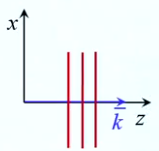
\includegraphics[scale=0.45]{ch2/image7.png}
\captionof{figure}{ }
\end{wrapfigure}
Or, il n'y a pas de dépendance en $x$ et $y$ comme le montre le schéma ci-contre. Avoir 
une composante selon $y$, ici $A_y$ n'implique pas une dépendance en $y$! Dès lors, 
seule la dérivée par rapport à $z$ est non-nulle. On en tire
\begin{equation}
iA_zke^{ikz}e^{-i\omega t} = 0\qquad \forall z,t
\end{equation}
Il en résulte que $A_z = 0$. Conclusion : le champ électrique est toujours transverse à 
l'axe $z$ pour une onde se déplaçant sur ce même axe.\\

Revenons à la description mathématique de la SG des EDP de Maxwell. Rappelons la \textbf{contrainte 
sur les modes de Fourier} 
\begin{equation}
k = \dfrac{\omega}{c}
\end{equation}
Le vecteur d'onde doit obligatoirement se balader sur une sphère :
\begin{equation}
k_x^2+k_y^2+k_z^2 = k^2 = \dfrac{\omega^2}{c}
\end{equation}
Rentrons cette contrainte dans l'expression de $E$. Or, nous n'avons que trois dimension : on 
fait le choix d'exprimer $k_z$ en fonction de la contrainte :
\begin{equation}
k_z = \sqrt{k^-k_x^2-k_y^2}
\end{equation}
Si $k_z$ satisfait cette relation, c'est gagné. Pour être solution, il faut que le spectre ai 
la forme particulière définie ci-dessous, qui ne dépend plus de $k_z$ la variable ayant été 
"sacrifiée" :
\begin{equation}
\tilde{E}(k_x,k_y,k_z,\omega) = \tilde{E}(k_x,k_y,\omega)\delta\left(k_z-\sqrt{k^-k_x^2-k_y^2}\right)
\end{equation}
où l'on introduit le delta de Dirac : si le spectre est limité à des spectres de cette forme là, 
d'office ce sera solution des équations de Maxwell\footnote{C'est une façon mathématique d'imposer 
la valeur de $k_z$.}. En substituant dans mon équation $\iiiint$, une des intégrales sera simplifiée 
par le delta de Dirac.
\begin{equation}
E(x,y,z,t) = \iiint_{-\infty}^\infty \tilde{E}(k_x,k_y,\omega) e^{ik_xx}e^{ik_yy}e^{i 
\sqrt{k^-k_x^2-k_y^2} z}e^{-i\omega t}\ dk_xdk_yd\omega
\end{equation}
Ce qui n'est rien d'autre que la solution générale des équations de Maxwell. Nous allons nous limiter 
à des ondes monochromatiques, c'est à dire pour un seul $\omega_0$. On se limite ainsi à un spectre 
spatial pour une fréquence donnée
\begin{equation}
\tilde{E}(k_x,k_y,\omega) = A(k_x,k_y)\delta(\omega-\omega_0)
\end{equation}
Notre intégrale triple devient
\begin{equation}
E(x,y,z,t) = \iint_{-\infty}^\infty A(k_x,k_y) e^{ik_xx}e^{ik_yy}e^{i 
\sqrt{k^-k_x^2-k_y^2} z}\ dk_xdk_ye^{-i\omega_0 t}
\end{equation}
où $\omega$ n'apparaît plus : il est caché dans la définition de $k$. On considère ici des ondes 
monochromatiques, on va dès lors s'affranchir du caractère temporel qui ne nous intéresse pas ici. 
Soit 
\begin{equation}
E(x,y,z,t) = a(x,y,z)e^{-i\omega_0t}
\end{equation}
où $a$ est l'amplitude indépendante du temps. On a donc
\begin{equation}
a(x,y;z) = \iint_{-\infty}^\infty A(k_x,k_y) e^{ik_xx}e^{ik_yy}e^{i 
\sqrt{k^-k_x^2-k_y^2} z}\ dk_xdk_y
\end{equation}
où $k^2 = \omega_0^2/c^2$. Ceci est à coup sur une solution des équations de Maxwell. Allégeons 
les notations : $k_x=\rho, k_y=\sigma, k_z=\beta=\sqrt{k^2-\rho^2-\sigma^2}$ pour avoir
\begin{equation}
a(x,y;z) = \iint_{-\infty}^\infty A(\rho,\sigma)e^{i\rho x}e^{i\sigma y} e^{i\sqrt{k^2-\rho^2-
\sigma^2}z}\ d\rho d\sigma
\end{equation}
Il s'agit d'une intégrale de Fourier, une combinaison linéaire d'onde plane qui ont certaines 
amplitudes qui représentent le spectre du champ. Il s'agit de l'expression d'une \textit{solution 
générale des équations de Maxwell pour une onde monochromatique}, le point de départ de la 
théorie de diffraction.


\newpage
\section{Diffraction et transformée de Fourier}
Histoire de nous habituer aux notations, reprenons la définition de la transformée de Fourier
\begin{equation}
F(\rho) = \int_{-\infty}^\infty f(x)e^{-i\rho x}\ dx
\end{equation}
\danger Il y a un signe négatif. Ce signe ne change physiquement rien, il faudra simplement 
inverser le signe de la transformée inverse. Il faut juste remarquer que le $i$ de l'exponentielle 
n'a pas le même signe dans la partie temporelle et spatiale : pour le temporelle, on utilise un 
moins et pour les variation spatiales un plus\footnote{Confusion, à éclaircir}. La transformée 
inverse vaudra alors
\begin{equation}
f(x) = \dfrac{1}{2\pi}\int_{-\infty}^\infty F(\rho)e^{i\rho x}\ d\rho = TF^{-1}[F(\rho)]
\end{equation}
Il faut remarquer que $a(x,y;z)$ est une transformée inverse. L'idée est que comme nous ne nous 
mesurerons jamais de valeur précise, il n'est pas utile de garder le facteur $1/2\pi$.\\

On remarque que le rôle de $z$ est différente des autres variables, les bornes d'intégrations 
ne portent pas sur lui : il n'apparaît que comme un simple paramètre. Il s'agit donc bien d'une 
fonction de $x$ et $y$. On remarque que l'on calcule la transformée inverse d'une fonction dans 
l'expression de $a(x,y;z)$ :
\begin{equation}
A(\rho,\sigma)e^{i\sqrt{k^2-\rho^2-\sigma^2}z}
\end{equation}
Il s'agit du \textit{spectre de Fourier} de la distribution transverse du champ en une valeur $z$, 
$a(x,y;z)$. Les $\rho,\sigma$ sont les fréquences spatiales. On peut ainsi écrire
\begin{equation}
a(x,y;z) = TF^{-1}\left[ A(\rho,\sigma)\underbrace{e^{i\sqrt{k^2-\rho^2-\sigma^2}z} }_{(*)}\right]
\end{equation}
Commençons l'étude en $z=0$ (C.I., connue)
\begin{equation}
a(x,y;z) = TF^{-1}\left[ A(\rho,\sigma) \right]\quad \Rightarrow \quad A(\rho,\sigma) = TF[
a(x,y;0)]
\end{equation}
On remarque que ceci n'est rien autre que le spectre de la transformée de Fourier de la distribution 
initiale. Le problème de diffraction est que connaissant la distribution initiale, on veut connaître 
la distribution $a(x,y;z)$ pour tout $z$. Si $z\neq0$, un facteur exponentiel supplémentaire apparaît 
: ce n'est rien d'autre que le \textbf{propagateur} $(*)$ de spectre. Le spectre initial est multiplié 
par un simple facteur de phase, une sorte de phaseur. Hélas, s'exprimer dans le spectre ne donne pas 
grand chose, le problème est la conversion spatiale.\\


Intéressons-nous avant tout à l'interprétation physique de la S.G., rappelée ici
\begin{equation}
a(x,y;z) = \iint_{-\infty}^\infty A(\rho,\sigma)e^{i\rho x}e^{i\sigma y} e^{i\sqrt{k^2-\rho^2-
\sigma^2}z}\ d\rho d\sigma
\end{equation}
Posons $\beta = \sqrt{k^2-\rho^2-\sigma^2}$
\begin{equation}
a(x,y;z) = \iint_{-\infty}^\infty A(\rho,\sigma)e^{i(\rho x + \sigma y + \beta z)}\ d\rho d\sigma
\end{equation}
On peut alors dire que le phaseur a une phase $\varphi \rho x + \sigma y + \beta z$. Si on considère 
cette phase constante, on considère le lieu des points vérifiant 
\begin{equation}
\varphi \rho x + \sigma y + \beta z = 2m\pi
\end{equation}
Il s'agit d'une équation de plan dont $\rho,\sigma$ et $\beta$ sont les cosinus directeur, les 
composantes du vecteur $k$. Ce phaseur n'est qu'une onde plane qui se propage avec un certain 
angle par rapport à l'axe $z$. Analysons l'intégrale dans sa globalité en faisant passé le 
faisceau laser par une fonction fenêtre (une fente infinie en $y$) :
\begin{equation}
\left\{\begin{array}{ll}
a(x';0) = a_0 & \text{ si } |x'| < l\\
a(x';0) = 0 & \text{ si } |x'| > l
\end{array}\right.\quad \Rightarrow\quad A(\rho) = 2l\ \text{sinc}(l\rho)
\end{equation}


\begin{wrapfigure}[7]{l}{3cm}
\vspace{-4mm}
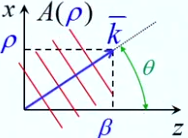
\includegraphics[scale=0.45]{ch2/image8.png}
\captionof{figure}{ }
\end{wrapfigure}
Admettons que l'on rentre le spectre dans l'intégrale, on remarque que pour des valeurs de $z>0$, 
le champ peut s'exprimer comme une sorte d'onde plane. Chaque valeur de $\rho$ représente un certain 
angle $\theta$ (projection sur $x$) et à chaque valeur de $\rho$ est associé une certaine amplitude : 
a chaque angle est associé une amplitude. Les équations de Maxwell (ici, sa solution) dit que l'on 
peut représenter par une somme d'onde plane dont l'amplitude est donnée par la transformée de 
Fourier.\\

Pour des $z>0$, on a une ensemble d'onde plane dont l'amplitude est donnée par la transformée de 
Fourier de la condition initiale : $\rho$ représente l'angle qui est $\theta = \arcsin(\rho/k)$. 
On a bien une somme d'onde plane qui donne lieu au phénomène de diffraction. Passons en revue 
quelques exemples triviaux.
\begin{enumerate}
\item Onde plane en $z=0 : a(x,y;0) = a_0$.\\
Le spectre recherché est le spectre de la condition initiale, c'est-à-dire la constante $a_0$\footnote{
$A(\rho) = \int_{-\infty}^\infty a_0e^{-i\rho x}\ dx = 2\pi a_0\delta(\rho)$}
\begin{equation}
A(\rho,\sigma) = TF[a(x,y;0)] = a_0\delta(\rho,\sigma)
\end{equation}
Après substitution
\begin{equation}
a(x,y;z) = a_0\iint_{-\infty}^\infty \delta(\rho,\sigma)e^{i\rho x}e^{i\sigma y} e^{i\sqrt{k^2-\rho^2-
\sigma^2}z}\ d\rho d\sigma
\end{equation}
Dès lors
\begin{equation}
a(x,y;z) = a_0e^{ikz}
\end{equation}
Ce qui est bien la réponse attendue. Il n'y a pas de diffraction, c'est un "mode de propagation" qui 
est invariant.
\item Onde plane inclinée selon $x = a(x,y;0) = a_0e^{i\rho_0x}$.\\
Ceci représente bien une onde avec un certain angle car $\rho_0 = l\sin\theta_0$. Après 
substitution (on choisit $\sigma=0$).
\begin{equation}
A(\rho,\sigma) = a_0\int e^{i\rho_0x}e^{-i\rho x}\ dx \int e^{-i\sigma y}\ dy
\end{equation}
On obtient le produit de deux Dirac, noté 
\begin{equation}
A(\rho,\sigma) = a_0\delta(\rho-\rho_0,\sigma)
\end{equation}
On retrouve une onde plane qui ne sera pas non plus modifiée par sa propagation
\begin{equation}
a(x,y;z) = a_0e^{i\rho_0x}e^{i\sqrt{k^2-\rho_0^2}z}
\end{equation}
Notons que $\beta_0 = k\cos\theta_0$. Les fronts d'onde seront les lieux de phase 
constantes
\begin{equation}
\varphi = k\sin\theta_0x + k\cos\theta_0 z = 2m\pi
\end{equation}
Un mode de Fourier est une onde plane, il s'agit de quelque chose qui ne se déforme pas.

\item Modulation harmonique transverse : $a(x,y;0) = a_0\cos(\rho_0x)$.\\
On retrouvera le même résultat si on se souvient que l'on peut écrire
\begin{equation}
a(x,y;0) = a_0\frac{e^{i\rho_0x}+e^{-i\rho_0x}}{2}
\end{equation}
Le spectre vaut
\begin{equation}
A(\rho,\sigma) = a_0\frac{\delta(\rho-\rho_0,\sigma)+\delta(\rho+\rho_0,\sigma)}{2}
\end{equation}
Le spectre est composé de deux delta de Dirac qui sélectionneront deux $\rho_0$ et 
$\sigma$ sera toujours bien nul:
\begin{equation}
a(x,y;z) = a_0\cos(\rho_0x)e^{i\sqrt{k^2-\rho_0^2}z}
\end{equation}
Il s'agit d'un autre mode. Le cosinus n'est la somme de deux ondes planes : une se 
déplaçant à un angle $\theta_0$ et l'autre avec un angle $-\theta_0$.

\item Diffraction par une fente infinie. En $z=0$ :
\begin{equation}
\left\{\begin{array}{ll}
a(x;0) = a_0 & \text{ si } |x| < l\\
a(x;0) = 0 & \text{ si } |x| > l
\end{array}\right.
\end{equation}
On considère une onde plane sur un écran qui va l'absorber sauf sur une largeur $2l$. 
Réduisons le problème en $2D$ ($x$ et $z$- : rien ne change en y, la fente est infinie.  
La transformée de Fourier est bien connue
\begin{equation}
A(\rho) = 2l\ sinc(\rho l)\qquad a_0=1
\end{equation}
Ci-dessous, la densité spectrale du spectre $|A(\rho)|^2$. 
\begin{center}
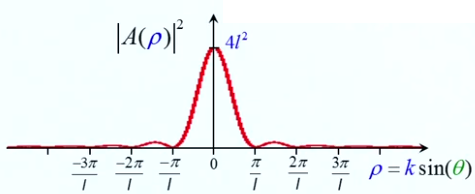
\includegraphics[scale=0.45]{ch2/image9.png}
\captionof{figure}{L'angle en abscisse (indirect) est celui de propagation. Pour une certaine 
direction, ceci donne l'amplitude correspondante.}
\end{center}
Cette fois-ci, la fonction est 
moins triviale : on ne calculera pas on se contentera de la physique. Si l'on place un 
détecteur, un certain $\rho$ va sélectionné un certain $\theta$ et cette valeur donne une 
certaine amplitude. On tombe sur une difficulté conceptuelle : on trouve la valeur de $k$ 
puis $\rho$ dépasse $k$ ; on recherche l'arc dont le sinus est supérieur à 1\footnote{$\theta =
\arcsin\frac{\rho}{k}$}.\\

Regardons le problème de la diffraction
\begin{equation}
a(x;z) = \int 2l\ \text{sinc}(l\rho)e^{i\sqrt{k^2-\rho_0^2}z}e^{i\rho x}\ d\rho
\end{equation}
A cause des bornes d'intégration, nous aurons d'office des valeurs de $\rho$ dépassant 
$k$. Passons outre et calculons :
\begin{equation}
\text{Si } \rho > k\quad \text{alors}\quad \beta = \sqrt{k^2-\rho^2} = i\sqrt{\rho^2-k^2} = 
i\alpha
\end{equation}
Ceci implique que l'exponentielle imaginaire présente dans $a(x;z)$ devient réelle :
\begin{equation}
e^{i\beta z} = e^{-\alpha z}
\end{equation}
On a ce que l'on appelle des \textbf{ondes évanescentes} : plutôt que d'avoir un comportement 
périodique à un comportement amorti. Ce que l'on va faire, c'est séparer l’intégrale en deux 
parties :
\begin{equation}
a(x;z) = \int_{-k}^k  2l\ \text{sinc}(l\rho)e^{i\sqrt{k^2-\rho_0^2}z}e^{i\rho x}\ d\rho + 
\int_{|\rho|>k}  2l\ \text{sinc}(l\rho)e^{-\sqrt{k^2-\rho_0^2}z}e^{i\rho x}\ d\rho
\end{equation}
Le deuxième terme somme des ondes évanescentes. En $z$, elles évoluent en exponentielles 
négatives. Quelle est cette absorption ? Il s'agit d'un phénomène de réflexion (il représente 
des photons qui passent l'écran et retournent de la ou ils viennent). 

\begin{center}
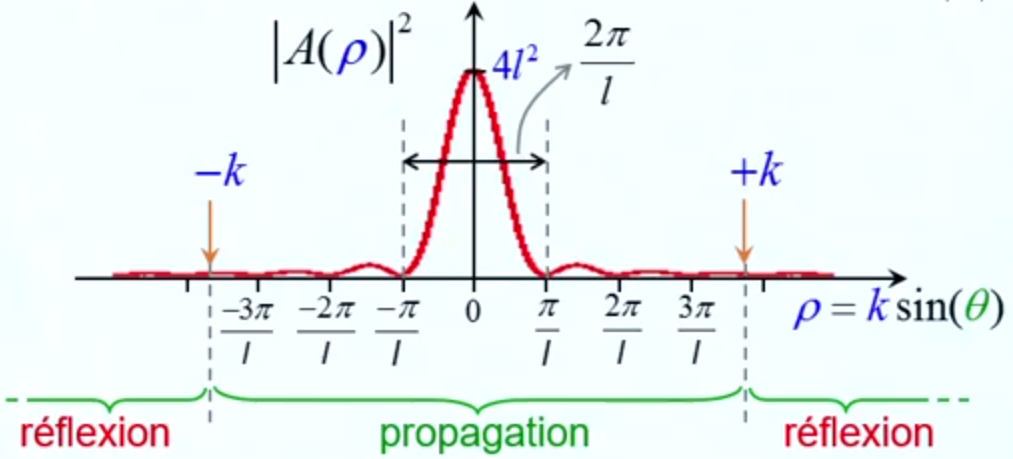
\includegraphics[scale=0.25]{ch2/image10.png}
\captionof{figure}{ }
\end{center}
Par simplification, 
on ne va s'arranger pour qu'elles soient négligeables. Pour se faire, analysons le spectre. 
La fonction sinus cardinal a un lobe principal : toute l'énergie est proche de l'origine. Nous 
allons travailler de sorte que les objets diffractant vérifient
\begin{equation}
\dfrac{2\pi}{l} \ll k = \dfrac{2\pi}{k}
\end{equation}
A ce moment la, le spectre est fort ramené à l'origine de sorte à ce que les ondes évanescentes 
soient négligées. Autrement dit
\begin{equation}
\int_{|\rho|>l} |A(\rho)|^2\ d\rho \ll \int_{-k}^{+k} |A(\rho)|^2\ d\rho
\end{equation}
Ce qui exprime que le spectre soit centrée sur l'origine et très étroit. Il faut dès lors que 
les objets diffractant sont significativement plus grand que la longueur d'onde : $\lambda \ll l$.\\

Le calcul de l'intégrale n'est pas évident (le facteur de phase gène). Nous allons utiliser 
l'approximation faite pour les ondes évanescentes :
\begin{equation}
\rho \approx \dfrac{2\pi}{l} \ll k
\end{equation}
On va pouvoir approximer le propagateur permettant de  ce cas, mais ceci est l'objet de la 
suivante section.
\end{enumerate}

\newpage
\section{Formule de diffraction de Fresnel}
Nous nous attarderons ici à reconstruire la fameuse formule de diffraction proposée par 
Fresnel sans se baser sur la transformée de Fourier (juste naissant) et les équations 
de Mawell (n'existant pas encore). Cependant, dans le cadre de ce cours, nous utiliserons 
ces deux outils.\\

Repartons de l'approximation de la solution générale des équations de Maxwell (on retrouve 
bien la contrainte sur les modes de Fourier)
\begin{equation}
a(x,y;z) = \iint_{-\infty}^\infty A(\rho,\sigma)e^{i\rho x}e^{i\sigma y} e^{i\sqrt{k^2-\rho^2-
\sigma^2}z}\ d\rho d\sigma
\end{equation}

\begin{wrapfigure}[8]{l}{9.5cm}
\vspace{-4mm}
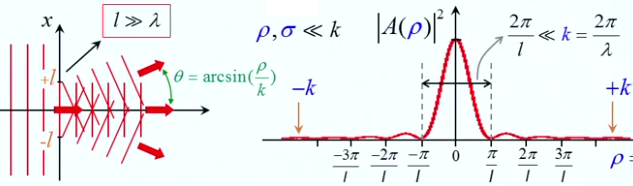
\includegraphics[scale=0.4]{ch2/image11.png}
\captionof{figure}{ }
\end{wrapfigure}
Nous allons ici approcher l'expression du propagateur. Une onde plane arrivée sur un écran 
percé. Chacune de ces ondes possédant un certain poids ($A$) se propage avec un certain 
angle ($\rho$ par rapport à $x$ et $\sigma$ par rapport à $y$). Nous travaillons dans la 
limite $\lambda \ll l$ pour négliger les ondes évanescentes de sorte à ce que les seules 
valeurs significatives\footnote{La pondération, c'est-à-dire l'amplitude $A$, n'est 
significative que pour les valeurs de $\rho$ proche de l'origine : $\rho,\sigma \ll k$} de 
$\rho$ soient incluent dans $\left[\frac{-\pi}{l};\frac{\pi}{l}\right]$.\\

\danger Le spectre limite les valeurs de $\rho$ et $\sigma$, ne pas confondre avec les 
(grandes) bornes d'intégration : le spectre sera bien toujours étroit et donc notre 
fonction est large.\\

Intéressons-nous à l'\textit{approximation paraxiale} : petits angles $\rho,\sigma\ll k$. 
En effet, lorsque $\rho,\sigma\ll k$ on travaille avec un arcsinus très faible, d'où le 
\textit{petits angles}. Ceci va permettre d'éliminer la racine, bien gênante dans notre 
S.G.
\begin{equation}
\beta = \sqrt{l^2-\rho^2-\sigma^2} = k\sqrt{1-\dfrac{\rho^2}{k^2}-\dfrac{\sigma^2}{k^2}}
\end{equation}
On peut dès lors utiliser l'approximation de McLaurin $\sqrt{1+\epsilon} \approx 1+\frac{1
}{2}\epsilon$ :
\begin{equation}
\beta \approx k\left[1-\dfrac{1}{2}\frac{\rho^2}{k^2}-\dfrac{1}{2}\dfrac{\sigma^2}{k^2}\right] =
k-\dfrac{1}{2}\dfrac{\rho^2}{k}-\dfrac{1}{2}\dfrac{\sigma^2}{k}\qquad\qquad\beta \in\mathbb{R}
\ \forall (\rho,\sigma)
\end{equation}
\begin{wrapfigure}[8]{r}{4cm}
\vspace{-4mm}
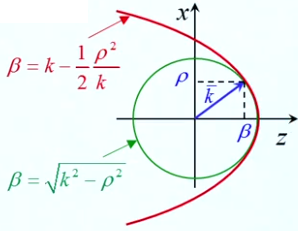
\includegraphics[scale=0.4]{ch2/image12.png}
\captionof{figure}{ }
\end{wrapfigure}
Le $\beta$ (la composante en $z$ du vecteur d'onde) obtenu est toujours réelle : la possibilité 
d'avoir des ondes évanescentes à été éliminée. Nous avons donc remplacé la contrainte sur 
les modes de Fourier (le vecteur d'onde devant se déplacer sur une sphère) a été changée en 
une contrainte de type parabolique. Ceci n'est valable que si la distribution angulaire est 
limitée ce qui n'est vrai que si la taille de l'objet est significativement grande devant la 
longueur d'onde.\\
Effectuons cette approximation par substitution :
\begin{equation}
a(x,y;z) = \iint_{-\infty}^\infty A(\rho,\sigma)e^{i\rho x}e^{i\sigma y} e^{i\frac{\rho^2}{2k}z
-i\frac{\sigma^2}{2k}z}\ d\rho d\sigma\ e^{ikz}
\end{equation}
Ceci est une simplification considérable, il va être possible de traiter ce terme de phase. Il 
suffit pour cela de remarquer que cette intégrale n'est que la transformée de Fourier inverse 
du spectre initial multiplié par le propagateur
\begin{equation}
a(x,y;z) = TF^{-1}\left[A(\rho,\sigma)e^{-i\frac{z}{2k}(\rho^2+\sigma^2)}\right]e^{ikz}
\end{equation}
Le facteur de phase étant quadratique, il est traitable analytiquement. Simplifions le problème 
en considérant que rien ne se passe en $y$ (le spectre est une delta de Dirac en $\sigma$) :
\begin{equation}
a(x;z) = TF^{-1}\left[A(\rho)\underbrace{e^{-\frac{z}{2k}\rho^2}}_{H_z(\rho)}\right]e^{ikz}
\end{equation}
On peut considérer que notre plaque percée obéit à la fonction fenêtre, suffisamment large devant 
la longueur d'onde\footnote{$z$ est un paramètre dans cette analyse.}. Plus proprement :
\begin{equation}
a(x;z) = TF^{-1}[A(\rho)H_z(\rho)]e^{ikz}
\end{equation}
Cette écriture nous permet d'utiliser le théorème de convolution de Fourier
\begin{equation}
a(x;z) = TF^{-1}[A(\rho)]\otimes TF^{-1}[H_z(\rho)]\ e^{ikz}
\end{equation}
Ou encore
\begin{equation}
a(x;z) = a(x;0)\otimes h_z(x)\ e^{ikz}
\end{equation}
où $a(x;0)$ est le champ initial, à l'endroit du plan diffractant. Avec la transformée de 
Fourier inverse (pour le peu que l'on intègre sur $\rho$) :
\begin{equation}
h_z(x) = \int e^{-i\frac{z}{2k}\rho^2}\ e^{i\rho x}\ d\rho
\end{equation}
Les tables mathématiques peuvent directement nous donner la solution de cette intégrale
\begin{equation}
h_z(x) = \sqrt{\frac{2k}{z}}\ e^{-i\dfrac{\pi}{4}}\ e^{i\dfrac{k}{2z}x^2}
\end{equation}
Ceci étant fait, explicitons la convolution à effectuer
\begin{equation}
a(x;z) = \int a(x':0)h_z(x-x')\ dx'\ e^{ikz}
\end{equation}
Après substitution
\begin{equation}
a(x;z) = \sqrt{\frac{2k}{z}}\int a(x';0) \ e^{-i\dfrac{\pi}{4}}\ e^{i\dfrac{k}{2z}(x-x')^2}\ 
dx'
\end{equation}
Il est aisé d'en dériver le résultat à deux dimensions transverses
\begin{equation}
h_z(x,y) = \sqrt{\frac{2k}{z}}\ e^{-i\dfrac{\pi}{4}}\ e^{i\dfrac{k}{2z}x^2} \times 
\sqrt{\frac{2k}{z}}\ e^{-i\dfrac{\pi}{4}}\ e^{i\dfrac{k}{2z}y^2}
\end{equation}
Après substitution
\begin{equation}
a(x,y;z) = \frac{2k}{z}\int a(x',y';0)\ e^{i\dfrac{k}{2z}(x-x)^2}\
 e^{i\dfrac{k}{2z}(y-y')^2}\ dx'dy'\ e^{-i\dfrac{\pi}{2}}\ e^{ikz}
\end{equation}
Ne faisant ici que du qualitatif, nous pouvons nous débarrasser des constantes. Intéressons
nous à cette fonction dont nous effectuons la convolution en incluant cette fois-ci le facteur 
de phase (la convolution ne portant que sur $x,y$ cela ne change rien)
\begin{equation}
a(x,y;z) = a(x,y:z)\otimes\left(h_z(x,y)\ e^{ikz}\right)
\end{equation}
où l'on s'intéresse à 
\begin{equation}
h_z(x,y)\ e^{ikz} = \frac{k}{z}\ e^{i\dfrac{k}{2z}(x^2+y^2)}\ e^{ikz}
\end{equation}
Qu'est ce que cette fonction? Nous savons qu'il s'agit de la fonction permettant de décrire 
le champ diffracté. C'est intéressant, mais qu'est ce qui permet de faire ça? Analysons la 
phase (quadratique, voir même parabolique) de ce terme
\begin{equation}
\varphi = \dfrac{k}{2z}x^2+\dfrac{k}{2z}y^2+kz
\end{equation}
Analysons la répartition de champ d'une onde sphérique $\frac{1}{r}e^{ikr}$ décrite en $kr$ 
où $k$ est un \textbf{nombre} d'onde (et pas un vecteur). On s'intéresse ici à la phase de 
cette onde : exprimons les lieux de phases constantes ou, autrement dit, les fronts d'ondes
\begin{equation}
\varphi = kr = 2m\pi
\end{equation}

\begin{wrapfigure}[8]{r}{4cm}
\vspace{-4mm}
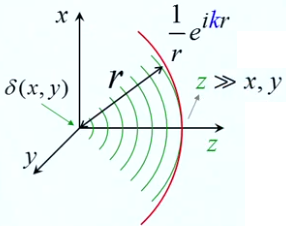
\includegraphics[scale=0.4]{ch2/image13.png}
\captionof{figure}{ }
\end{wrapfigure}
où $r = \sqrt{x^2+y^2+z^2}$. En se plaçant dans des conditions paraxiales (très proche de 
l'axe $z$) : $x,y \ll z$. On se propose donc d'analyser la phase d'une onde sphérique dans 
la zone ou les conditions paraxiales sont réunies. On peut approximer la racine
\begin{equation}
r\sqrt{1+\dfrac{x^2}{z^2}+\dfrac{y^2}{z^2}} \quad \Rightarrow \quad\left[1+\dfrac{x^2}{2z^2}+
\dfrac{y^2}{2z^2}\right]
\end{equation}
Dès lors
\begin{equation}
\varphi = kr = kz+ \dfrac{k}{2z}x^2+\dfrac{k}{2z}y^2 = 2m\pi
\end{equation}
Il s'agit d'un paraboloïde, c'est bien une approximation parabolique de fronts d'onde 
sphériques, généralement générés par des petites sources ponctuelles d'ondes électromagnétiques 
assimilables à des delta de Dirac, le champ magnétique vibre en un point de l'espace et 
génère une onde sphérique.\\

\begin{wrapfigure}[11]{l}{3.5cm}
\vspace{-5mm}
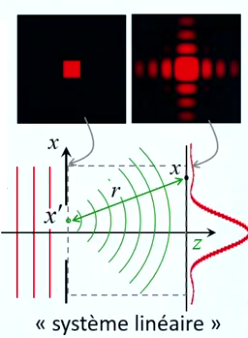
\includegraphics[scale=0.4]{ch2/image14.png}
\captionof{figure}{ }
\end{wrapfigure}
Revenons à notre problème. Le champ initial est la fameuse fonction fenêtre. Après une certaine 
distance parcourue, on récupère un certain profil donne par (ici) un profil à deux dimensions. 
Nous pouvons voir ça comme un système linéaire (en effet, des ondes rentrent et en sortent 
modifiées). Nous avions déjà rencontré ce système en  utilisant le principe de superposition, 
les équations de Maxwell étant linéaires dans le vide\footnote{On peut voir toute onde comme 
une combili d'ondes harmoniques}. \\

Le champ est un produit de convolution du champ d'entrée avec une fonction de phase quadratique qui 
ne représente rien d'autre qu'une phase sphérique. Nous voyons une sommes d'ondes sphériques en 
approximation paraboliques mis sous la forme d'une convolution. En effet, le $x-x'$ représente le 
fait que l'onde ne vient plus de l'origine (comme dans $h_z$) mais désigne un point qui n'est plus 
à l'origine mais au point $(x',y')$.
\begin{equation}
r = \sqrt{(x-x')^2+z^2}
\end{equation}
En approchant ceci par l'approximation parabolique
\begin{equation}
r \approx z+\dfrac{(x-x')^2}{2z}
\end{equation}
Ceci est précisément ce qui apparaît dans notre convolution\footnote{Débarrassée des constantes.} :
\begin{equation}
a(x,y;z) = \frac{k}{z}\int a(x',y';0)\ e^{i\dfrac{k}{2z}(x-x)^2}\
 e^{i\dfrac{k}{2z}(y-y')^2}\ dx'dy'\  e^{ikz}
\end{equation}

Nous ne travaillons finalement que avec la "\textit{réponse impulsionnelle}" du système où 
l'impulsion est cette source ponctuelle située en $(x',y')$. Nous avons en effet la réponse 
à une source ponctuelle (un delta, cette fois ci non temporel mais spatial) générant l'onde 
$h_z$ (l'onde sphérique approchée de façon parabolique) $\rightarrow$ réponse impulsionnelle.\\


Un point source donne lieu à une certaine répartition de champ. La réponse globale s'obtient en 
prenant la convolution avec cette réponse, c'est-à-dire en considérant que chaque point a une 
certaine amplitude $a(x',y';0)$ : l'objet à une certaine amplitude et chaque de ces amplitude 
rayonne une onde sphérique partant de $(x',y')$ ou l'on a une certaine amplitude. \\

\begin{wrapfigure}[9]{l}{6.5cm}
\vspace{-5mm}
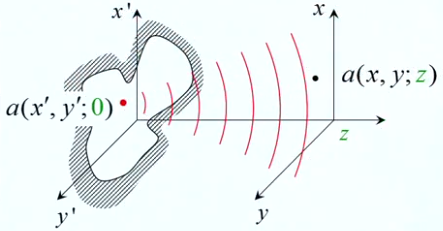
\includegraphics[scale=0.4]{ch2/image15.png}
\captionof{figure}{ }
\end{wrapfigure}
On retrouve le 
principe de Huygens : un écran laisse passé un trou laissant passé la lumière avec une certaine 
amplitude dépendant de $x'$ et $y'$. Chaque point de cet objet peut être considéré comme un point 
source générant une onde sphérique pouvant être approchée paraboliquement. En $z$, nous sommons 
(à travers l'intégrale) les champs de chacune de ces ondes sphériques. Nous avons une 
superposition d'onde sphérique d'amplitude donnée par l'amplitude de l'objet de départ : la 
figure de diffraction résultera des interférences entre toutes ces ondes sphériques (seulement une 
est représentée ci-contre).\\

Ceci est ainsi de la formule de diffraction de Fresnel, cette intégrale de Fresnel ne représente 
rien d'autre qu'une superposition d'ondelettes de Huygens.
\begin{equation}
a(x,y;z) = \frac{2k}{z}\int a(x',y';0)\ e^{i\dfrac{k}{2z}(x-x)^2}\
 e^{i\dfrac{k}{2z}(y-y')^2}\ dx'dy'\ e^{-i\dfrac{\pi}{2}}\ e^{ikz}
\end{equation}


Analysons les amplitudes des ondelettes de Huygens, ici en analysant leur amplitude. Considérons 
une de ces ondes, celle venant de l'origine ($x'=y'=0$) :
\begin{equation}
a(x,y;z) = \dfrac{k}{z}e^{i\dfrac{k}{2z}(x^2+y^2)}\ e^{ikz}
\end{equation}
Il s'agit de la fonction $h_z$ que nous avions précédemment\footnote{Pq?}



Nous avons une onde sphérique approchée par une onde parabolique dont le profil d'intensité 
(le module carré du champ) est donné par
\begin{equation}
I(x,y;z) = |a(x,y;z)|^2 \propto \dfrac{1}{z^2}
\end{equation}
Ceci peut paraître curieux car la décroissance réelle d'une onde est en $\frac{1}{r^2}$.
\begin{equation}
I(x,y;z) \propto \frac{1}{r^2}
\end{equation}
Pourquoi donc ? Il ne faut pas oublier que la notion d'intensité est locale : c'est la 
densité de flux énergétique de l'onde ($W/m^2$). S'il y a une certaine radiation la puissance 
totale s'obtient par l'intégration de cette radiation sur une sphère : on obtient la 
puissance radiée par la source (on obtient de $W$). La puissance rayonnée au travers de cette 
sphère est donnée par $4\pi r^2 I$ où $r$ est le rayon de la sphère sur laquelle on intègre. 
Or, cette intensité doit bien être constante (indépendante de $r$) : peu importe la sphère, 
la puissance émise de la source est constante, d'où la variation en $r^{-2}$.\\

\begin{wrapfigure}[9]{r}{5cm}
\vspace{-5mm}
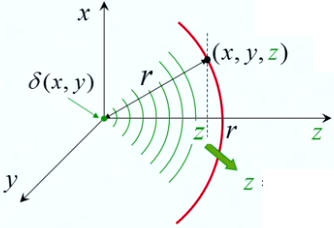
\includegraphics[scale=0.4]{ch2/image16.png}
\captionof{figure}{ }
\end{wrapfigure}
Or, nous obtenons $1/z^2$ et non pas $1/r^2$. Analysons pour cela l'onde sphérique en un 
point de coordonnée $(x,y,z)$ correspondant à un certain rayon : il y a une différence 
entre $z$ et $r$ (voir schéma ci-contre). Faisons la comparaison. Considérons $r$ dans le 
cadre de l'approximation paraxiale $x,y \ll z$ :
\begin{equation}
r = z+\frac{1}{2z}(x^2+y^2) + \mathcal{O}(2)
\end{equation}



En réalité, pour décrire cette onde, le front d'onde en $e^{ikz}$ a été approché : la 
sphère a été approché par une parabole, l'ordre un du développement a été gardé. Or, nous 
sommes passé de $1/r$ à $1/z$ car nous n'avons pas fait la même 
approximation. Pour la phase on considère que $r = z +\frac{1}{2z}(x^2+y^2)$ et pour l'amplitude 
on dit que $r=z$ (l'ordre un pour l'amplitude a été supprimé). Ceci peut paraître paradoxal, 
mais c'est parce que nous avons considéré 
\begin{equation}
\frac{1}{z^2}\approx\frac{1}{r^2}
\end{equation}
On peut se permettre de faire ça car une petite erreur sur la phase peut résulter en de 
grandes erreurs du profil diffracté. Mais si on se trompe sur la valeur de $r$ (petite 
erreur : $\delta r \approx 10^{-6}m\approx \lambda$) peut créer une erreur sur la phase 
de l'ordre de 100\% alors que sur l'amplitude, cela ne change quasiment rien. Il est donc 
tout à fait légitime de garder l'approximation d'ordre 1 pour évaluer la distance dans le 
terme de phase et de se contenter de l'approximation d'ordre 0 pour l'amplitude.



\newpage
\section{Formule de diffraction de Fraunhofer}
Pour établir cette nouvelle formule, repartons de la formule de diffraction de Fresnel
\begin{equation}
a(x,y;z) = \frac{k}{z}\int a(x',y';0)\ e^{i\dfrac{k}{2z}(x-x)^2}\
 e^{i\dfrac{k}{2z}(y-y')^2}\ dx'dy'\  e^{ikz}
\end{equation}
Rappelons l'interprétation physique de cette formule.
A partir de la connaissance du champ électromagnétique lumineux dans un certain plan 
($z=0$) on peut connaître le champ en toute position $z$ grâce à cette formule. Dans 
celle-ci nous retrouvons la phase des ondelettes de Huygens. Ce phaseur d'ondelette 
est multiplié par une amplitude puis on sommera tout via les intégrales. Intéressons-
nous à la phase de ces ondelettes où les carrés ont été développés
\begin{equation}
\varphi = kz + \frac{k}{2z}\left[x^2 + y^2 + x^{'2} + y^{'2} - 2xx'-2yy'\right]
\end{equation}
La diffraction de Fraunhofer fait un pas supplémentaire dans l'approximation de ces 
ondelettes : on va négliger les termes\footnote{Les axes en prim' sont ceux du repère 
attaché à l'objet diffractant.} $x^{'2}$ et $y^{'2}$ (mais on les garde au premier 
ordre). Pour se faire, nous allons limiter la taille de l'objet
\begin{equation}
x',y' \ll x,y
\end{equation}
En réalité, c'est la phase $\frac{kx^{'2}}{2z}$ que l'on choisi de négliger, c'est-à-dire
\begin{equation}
e^{i\dfrac{k}{2z}\|\vec{x'}\|^2_{\max}} \approx 1\qquad\Rightarrow\qquad \dfrac{k}{2z}\|
\vec{x'}\|^2_{\max}\ll 1
\end{equation}
où $\|\vec{x'}\|^2_{\max}$ est la plus grande distance depuis l'origine à l'extrémité 
de l'objet. Si ce facteur de phase est proche de l'unité, ce terme en prim' carré peut 
bien être supprimé. On peut écrire
\begin{equation}
\dfrac{k}{2}\|\vec{x'}\|^2_{\max} \ll z
\end{equation}
Or $k = \frac{2\pi}{\lambda}$, dès lors
\begin{equation}
\dfrac{\pi}{\lambda}\|\vec{x'}\|^2_{\max} \ll z
\end{equation}

\begin{wrapfigure}[9]{r}{7.5cm}
\vspace{-5mm}
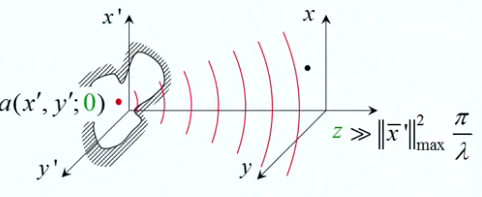
\includegraphics[scale=0.45]{ch2/image17.png}
\captionof{figure}{ }
\end{wrapfigure}
Si la distance $z$ est plus grande que la taille de l'objet au carré divisée par la longueur 
d'onde (le facteur pi ne change pas l'ordre de grandeur), cette approximation est bien valide
et on  parlera de \textit{zone de Fraunhofer}. Il ne reste que des termes linéaires dans notre 
phase
\begin{equation}
\varphi = kz + \frac{k}{2z}\left[x^2 + y^2 - 2xx'-2yy'\right]
\end{equation}
Après substitution
\begin{equation}
a(x,y:z) = \frac{k}{z}\int a(x',y';0) e^{i\frac{k}{2}(x^2+y^2)}e^{-i\frac{k}{z}(xx'+yy')}\ 
dx'dy'\ e^{ikz}
\end{equation}
En regroupant les termes de phases, on peut écrire
\begin{equation}
a(x,y:z)e^{ikz} e^{i\frac{k}{2}(x^2+y^2)} = \frac{k}{z}\int a(x',y';0) e^{-i\frac{k}{z}(xx'+yy')}\ 
dx'dy'\ 
\end{equation}
En séparant le terme de phase en deux
\begin{equation}
a(x,y:z) = \dfrac{k}{z} e^{ikz} e^{i\dfrac{k}{2}(x^2+y^2)} \underbrace{\int a(x',y';0) e^{-i\dfrac{k
}{z}xx'}e^{-i\dfrac{k}{z}yy'}\ dx'dy'}_{A\left(\frac{kx}{z},\frac{ky}{z}\right)}
\end{equation}
En posant $\rho = k/zx$ et $\sigma = k/zy$ on retrouve la définition de la transformée de Fourier 
$A(\rho,\sigma)$ : il s'agit de la transformée de Fourier du champ objet. Dès lors\\

\retenir{\textbf{Formule de diffraction de Fraunhofer}
\begin{equation}
a(x,y;z) = \dfrac{k}{z} e^{ikz} e^{i\dfrac{k}{2}(x^2+y^2)}\ A\left(\frac{kx}{z},\frac{ky}{z}\right)
\end{equation}
où $A$ est la transformée de Fourier du champ objet en $z=0$.}\ 

Ce qui n'est rien d'autre qu'un facteur de phase multiplié par un certain spectre aux variables 
un peu plus particulière que d'habitude. Le profil d'intensité sera ainsi directement 
proportionnel à la densité spectrale
\begin{equation}
I(x,y) \propto \left| \left(\frac{kx}{z},\frac{ky}{z}\right) \right|^2
\end{equation}

\begin{wrapfigure}[10]{l}{7cm}
\vspace{-5mm}
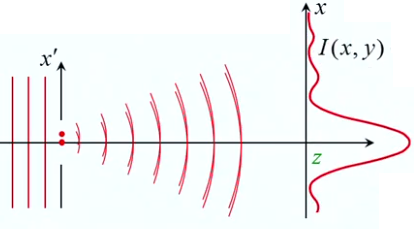
\includegraphics[scale=0.45]{ch2/image18.png}
\captionof{figure}{ }
\end{wrapfigure}
Intéressons-nous à l'interprétation physique de cette formule. Plutôt que de considérer le 
problème tridimensionnel des ondelettes de Huygens, revenons à un cas plus simple (une 
dimension transverse $x'$. Commençons par interpréter le premier facteur. Considérons 
"l'ondelette centrale" c'est-à-dire celle donnée par la formule de Fresnel en $x'=y'=0$ : 
dans ce cas, la phase est identique à celle présente dans le terme de hase de la 
formule de diffraction de Fraunhofer. On reconnaît donc l'ondelette de Huygens pour un 
point centré à l'origine. Ceci est normal, car à grande distance les deux sources 
ponctuelles ne semblent former qu'une de sorte à ce qu'à grande distance, les fronts d'
ondes soient superposés. La répartition de phase est très proche de celle de l'ondelette 
d'Huygens centrée à l'origine, avec le fameux décroissement en $1/z^2$.\\


\begin{wrapfigure}[10]{r}{7cm}
\vspace{-3mm}
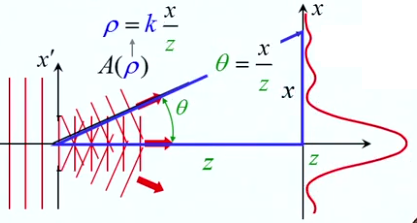
\includegraphics[scale=0.45]{ch2/image19.png}
\captionof{figure}{ }
\end{wrapfigure}
Le second terme, la modulation d'amplitude, est plus délicat à interpréter. Pour se faire, 
repartons du point de départ de l'établissement de la formule de diffraction de Fresnel :
\begin{equation}
a(x,y;z) = \iint_{-\infty}^\infty A(\rho,\sigma)e^{i\rho x}e^{i\sigma y} e^{i\sqrt{k^2-\rho^2-
\sigma^2}z}\ d\rho d\sigma
\end{equation}
Ce qui n'est rien d'autre que la S.G. de Maxwell. Passons à une dimension transverse (une 
delta pour le $\sigma$) $x'$ :
\begin{equation}
a(x;z) = \int A(\rho)e^{i\rho x} e^{i\sqrt{k^2-\rho^2}z}\ d\rho 
\end{equation}
De même, le résultat de Fraunhofer devient
\begin{equation}
I(x) \propto \left|A\left(\dfrac{kx}{z}\right)\right|^2
\end{equation}
Dans Fresnel, $A(\rho)$ est le spectre en $z=0$, chaque valeur de $\rho$ représentant une 
onde plane avec un certain angle ($\rho = k\sin\theta$, soit la projection en $x$ du 
vecteur d'onde)(comme nous travaillons à petit angle : $\rho = k\theta$). L'intensité à une 
certaine hauteur $x$ vient d'une onde possédant un certain angle $\theta$. On en tire
\begin{equation}
\tan \theta = \dfrac{x}{z}\qquad \rightarrow \qquad \rho = k\frac{x}{z}
\end{equation}

\begin{wrapfigure}[10]{l}{6.5cm}
\vspace{-3mm}
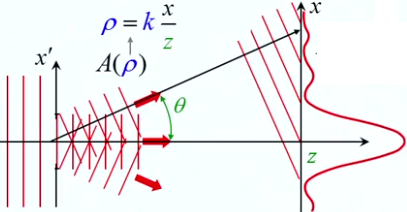
\includegraphics[scale=0.45]{ch2/image20.png}
\captionof{figure}{ }
\end{wrapfigure}
On sélectionne ainsi l'onde plane ayant pour valeur de $\rho = kx/z$. On comprend maintenant 
bien pourquoi on observe ce $A(kx/z)$. Hélas, sur notre schéma ci-dessous les ondes planes 
sont dessinées "limitées". Or, en réalité, elles ont bien une extension infinie ce qui rend 
l'interprétation physique bien moins satisfaisante. Du moins, c'est ce que l'on pourrait 
croire (que l'onde plane éclaire tout le plan) mais c'est faux (ouf!). Comment le justifier 
? Pourquoi n'éclaire-t-elle qu'un seul point ? Il faut aller plus loin dans l'interprétation. 
Pour se faire, il est nécessaire d'utiliser le \textit{théorème des phases stationnaires}.

	\subsection{Théorème des phases stationnaires}
	Nous allons appliquer ce théorème au calcul de l'intégrale de Fourier suivante
	\begin{equation}
	a(x;z) = \int A(\rho)\ e^{i\rho x}e^{i\sqrt{k^2-\rho^2}z}\ d\rho
	\end{equation}
	sur laquelle nous appliquer l'approximation paraxiale
	\begin{equation}
	\sqrt{k^2-\rho^2} = k-\frac{1}{2}\frac{\rho^2}{k}
	\end{equation}
	Après substitution
	\begin{equation}
	a(x;z) = \int A(\rho)\ e^{i\rho x}e^{-i\frac{z}{2k} z}\ d\rho\ e^{ikz}
	\end{equation}
	Intéressons-nous à la phase de cette intégrande 
	\begin{equation}
	\varphi(\rho) = \rho x - \dfrac{z}{2k}\rho^2
	\end{equation}
	
	\begin{wrapfigure}[15]{r}{4.5cm}
	\vspace{-3mm}
	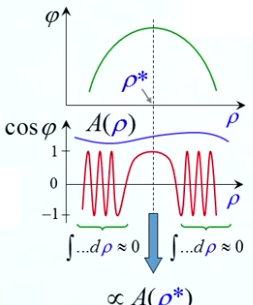
\includegraphics[scale=0.5]{ch2/image21.png}
	\captionof{figure}{ }
	\end{wrapfigure}
	Il s'agit d'une parabole, la dépendance de $\varphi$ en $\rho$ présente bien un 
	maximum. Regardons le phaseur (l'exponentielle de $i\varphi$). Représentons la 
	partie réelle de cette exponentielle (par facilité, mais n'oublions pas qu'il 
	existe une partie imaginaire). Au moment du maximum, $\varphi$ ne varie que peu 
	et l'on observe un état "stationnaire" du cosinus. Lorsque $\varphi$ varie 
	rapidement, on observe bien des oscillations rapide du cosinus. Comme nous avons 
	considéré un objet petit, le spectre sera forcément large. Or, nous avons le 
	produit du spectre par l'exponentielle imaginaire représentée par le cosinus. Dans 
	les zones de variation rapide, le produit sera approximativement nul, la seule 
	partie ayant une contribution notable est celle correspondant à une variation 
	lente du cosinus, donnant quelque chose de proportionnel au spectre (le cosinus 
	valant $\approx 1$). On nomme ci-contre $\rho^*$ la valeur pour laquelle nous 
	avons la stationarité de la phase, c'est-à-dire
	\begin{equation}
	\varphi'(\rho^*)=0\quad \Leftrightarrow\quad \rho^* = \dfrac{kx}{z}
	\end{equation}
	\newpage
	
		\begin{wrapfigure}[15]{l}{4.5cm}
%	\vspace{-3mm}
	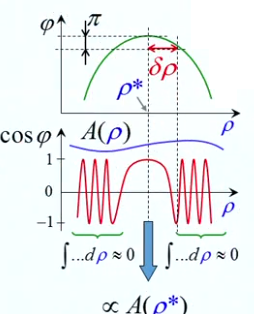
\includegraphics[scale=0.5]{ch2/image22.png}
	\captionof{figure}{ }
	\end{wrapfigure}
	On retrouve le résultat de Fraunhofer, $a(x;z) \propto A\left(\dfrac{kx}{z}
	\right)$. Il faut maintenant vérifier que nous sommes dans les conditions de 
	notre approximation. Considérons la phase stationnaire et descendons de $\pi$ (car 
	au déla, les oscillations sont rapides, le résultat du produit est nul). Ceci 
	correspond à une largeur $\delta \rho$ (la largeur de la fonction cosinus). Or, 
	il est possible d'évaluer ce $\delta\rho$ car nous avons connaissance de l'expression 
	de notre parabole
	\begin{equation}
	\dfrac{z}{2k}\delta\rho^2 = \pi\quad\Leftrightarrow\quad \delta\rho^2 = \dfrac{
	2\pi k}{z}
	\end{equation}
	Pour que le théorème des phases soit variable, il faut que le $\delta \rho$ soit 
	beaucoup plus petite que la variation du spectre (on considère que le spectre 
	est constant sur $\Delta \rho$ (extension spectrale suffisamment grande)
	\begin{equation}
	\delta\rho^2 = \dfrac{2\pi k}{z} \ll \Delta \rho^2
	\end{equation}
	Or, la largeur spectrale de notre fonction fenêtre vaut $2\pi/l$, on peut dire que 
	$\Delta \rho \approx \frac{2\pi}{\|\vec{x'}\|_{\max}}$. Dès lors
	\begin{equation}
	\dfrac{2\pi k}{z}\ll \dfrac{4\pi^2}{\|\vec{x'}\|_{\max}^2}
	\end{equation}
	En explicitant $k=2\pi/\lambda$, en simplifiant : $\frac{\|\vec{x'}\|^2_{\max}}{\lambda}
	\ll z$ ce qui est la zone de Fraunhofer ! Ce théorème est donc applicable.\\
	

\begin{wrapfigure}[10]{l}{6.5cm}
	\vspace{-3mm}
	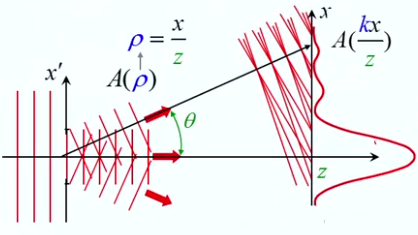
\includegraphics[scale=0.45]{ch2/image23.png}
	\captionof{figure}{ }
	\end{wrapfigure}	
Le théorème des phases stationnaires nous dit que si l'on observe $A\left(\dfrac{kx}{z}
\right)$ à un seul point (et non pas tout l'écran) c'est parce que en ce point la il va 
y avoir interférences constructives entre les ondes. Représentons une onde plane qui a une 
valeur de $\rho$ légèrement supérieure. Ces ondes ont des interférences constructives au 
point considéré et quelconques ailleurs : toutes les zones au $\rho$ proche vont 
construire un champ important au point $x$. Aux autre points, on sommes des champs aléatoires 
pour obtenir finalement zéro. C'est ce que dit notre théorème, nous n'avons interférences 
constructives que proche de $\rho \approx \rho^*$, le reste ne contribue pas.
	






































